\documentclass[10pt,twocolumn,letterpaper]{article}

\usepackage{cvpr}
\usepackage{times}
\usepackage{epsfig}
\usepackage{graphicx}
\usepackage{amsmath}
\usepackage{amssymb}

% Include other packages here, before hyperref.

% If you comment hyperref and then uncomment it, you should delete
% egpaper.aux before re-running latex.  (Or just hit 'q' on the first latex
% run, let it finish, and you should be clear).
\usepackage[breaklinks=true,bookmarks=false]{hyperref}

\cvprfinalcopy % *** Uncomment this line for the final submission

\def\cvprPaperID{****} % *** Enter the CVPR Paper ID here
\def\httilde{\mbox{\tt\raisebox{-.5ex}{\symbol{126}}}}

% Pages are numbered in submission mode, and unnumbered in camera-ready
%\ifcvprfinal\pagestyle{empty}\fi
\setcounter{page}{1}
\begin{document}

%%%%%%%%% TITLE
\title{Deep Audio Style Transfer}

\author{Durvesh Vedak\\
New York University\\
{\tt\small dvv223@nyu.edu}
% For a paper whose authors are all at the same institution,
% omit the following lines up until the closing ``}''.
% Additional authors and addresses can be added with ``\and'',
% just like the second author.
% To save space, use either the email address or home page, not both
\and
Karan Bhatia\\
New York University\\
{\tt\small kb3053@nyu.edu}
}


\maketitle
%\thispagestyle{empty}

%%%%%%%%% ABSTRACT
\begin{abstract}
“Style transfer” among images has recently emerged as a very
active research topic, fuelled by the power of convolution
neural networks (CNNs), and has become fast a very popular
technology in social media. This paper investigates the
analogous problem in the audio domain: How to transfer the
style of a reference audio signal to a target audio content?. We propose a framework for our task which uses a pretrained network to extract statistics characterizing the reference audio style followed by an optimization-based audio synthesis to modify the target content. In order to extract features of
interest, we investigate different architectures, such as pretrained
on other tasks, as done in image style transfer. Experimental
results on different types of audio signal confirm the potential
of the proposed approach.
\end{abstract}

%%%%%%%%% BODY TEXT
\section{Introduction}

\subsection{Inspiration from Neural Style Transfer}
Both visual texture synthesis, whose goal is to synthesize a
natural looking texture image from a given sample, and visual
texture transfer, which aims at weaving the reference texture
within a target photo, have been long studied in computer
vision \cite{Authors00002}. Recently, within the era of convolutional neural
networks (CNNs), these subjects have been revisited with
great success. In their seminal work, Gatys et al. \cite{Authors00001} exploit
the deep features provided by a pre-trained object recognition
CNN to transfer by optimization the “style” (mainly texture
at various scales and color palette) of a painting to a photograph
whose layout and structure are preserved. The result is
a pleasing painterly depiction of the original scene. This is
a form of example-based non-photorealistic rendering, which work of Gatys et al \cite{Authors00001}. has sparked a great deal of research, see
recent review on neural style transfer.

\subsection{Previous attempts on Audio Style Transfer}
Many of the related work in audio style transfer has been much inspired by the success of artistic style transfer.There were earlier attempts on audio style transfer using
CNN with 1 layer and 4096 filters. Ulyvamov and
Lebedev\cite{Authors00003} attempted this by converting raw audio to spectrogram
using short-time fourier transform and converting
back the output spectrogram to raw audio using Griffin Lim
algorithm \cite{Authors00004}.

\section{Related Work and References}
Ulyvamov and Lebedev\cite{Authors00003} attempted this by converting raw audio to spectrogram
using short-time fourier transform and converting
back the output spectrogram to raw audio using Griffin Lim
algorithm \cite{Authors00004}. An unusual approach taken by Ulyanov and
Lebedev is reshaping the 2D spectrogram (1 channel, with one dimension as time and the other as frequency) into an image with height 1, width as the number of timesteps in spectrogram, and the number of channels as the number of frequency bins in the original spectrogram. Instead of training the network, Grinstein\cite{Authors00005}
used a pretrained network (SoundNet) and hand-crafted
rules on human auditory perception. They found that SoundNet outperformed VGG-19, and that the shallow CNN significantly outperformed both large networks. Verma et al \cite{Authors00006} pre-trained an Alex-Net architecture \cite{Authors00007} on an instrument classification task and then applied the Gatys et al \cite{Authors00001}




\begin{figure*}
\begin{center}
\fbox{
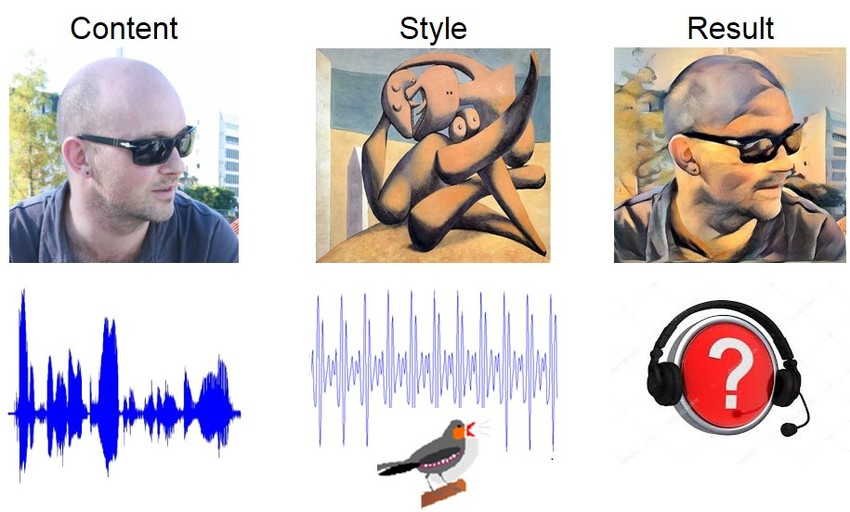
\includegraphics[scale=0.5]{analogy.png}
}
\end{center}
   \caption{Drawing analogy from example-based image stylisation}
\label{fig:short}
\end{figure*}

\section{Problem Identification and Proposed Method}
\subsection{Problems with existing method}
There has been much success with Neural Style transfer
on images where conventional CNN works well on 2-D
images. However, this method does not give satisfactory
results for audio style transfer. CNN’s are not suited for
capturing long term dependencies as in case of audio files.

One challenge posed in the comparison between visual images and spectrograms is the fact that visual objects and sound events do not accumulate in the same manner. To use a visual analogy, one could say that sounds are always “transparent” whereas most visual objects are opaque.

When encountering a pixel of a certain color in an image, it can most often be assumed to belong to a single object. Discrete sound events do not separate into layers on a spectrogram: Instead, they all sum together into a distinct whole. That means that a particular observed frequency in a spectrogram cannot be assumed to belong to a single sound as the magnitude of that frequency could have been produced by any number of accumulated sounds or even by the complex interactions between sound waves such as phase cancellation. This makes it difficult to separate simultaneous sounds in spectrogram representations.

In images, similar neighboring pixels can often be assumed to belong to the same visual object but in sound, frequencies are most often non-locally distributed on the spectrogram. Periodic sounds are typically comprised of a fundamental frequency and a number of harmonics which are spaced apart by relationships dictated by the source of the sound. It is the mixture of these harmonics that determines the timbre of the sound.

\subsection{Dataset}
For pre-training networks we will use dataset containing audio clips in .wav format. The dataset  contains 3-seconds music recording labelled by predominant class. We used a dataset downloaded from https://datahack.analyticsvidhya.com/contest/practice-problem-urban-sound-classification/ and used this dataset to train our deep model on audio spectrograms giving it the task of audio classification.

\subsection{Proposed Method}
Our proposed method will focus on improving the existing method for audio
style transfer i.e minimizing the loss between content
and output audio which will be sum of mean squared error
loss and the cost between Gram matrix of style and output
audio. Later we plan to improve the base model which will be CNN model by experimenting deeper CNN models to see if it captures the content and style audio features better than shallow Convolutional Neural Networks.
The inputs to this implementation of audio neural style transfer is 2 raw audio recordings (in formats such as .wav or .mp3) which are clipped to exactly 3 seconds in duration. One recording is designated as the content input and the other is designated as the style input. The final output of neural style transfer is a raw audio file (in .wav format) which has content features (such as melody)
from the content input and style features (such as instrumentation and duration of notes) from the
style input. 
To generate the synthesized outputs, we first convert the content and style audio to spectrograms via short-time fourier transform, yielding a 2 dimensional representation of the audio signal. We then use a pretrained neural network to extract content and style features from the content and style spectrograms, and then initialize the output spectrogram with the content and iteratively update the output until its content features match that of the content spectrogram and its style features match that of the style spectrogram.

\begin{figure*}
\begin{center}
\fbox{
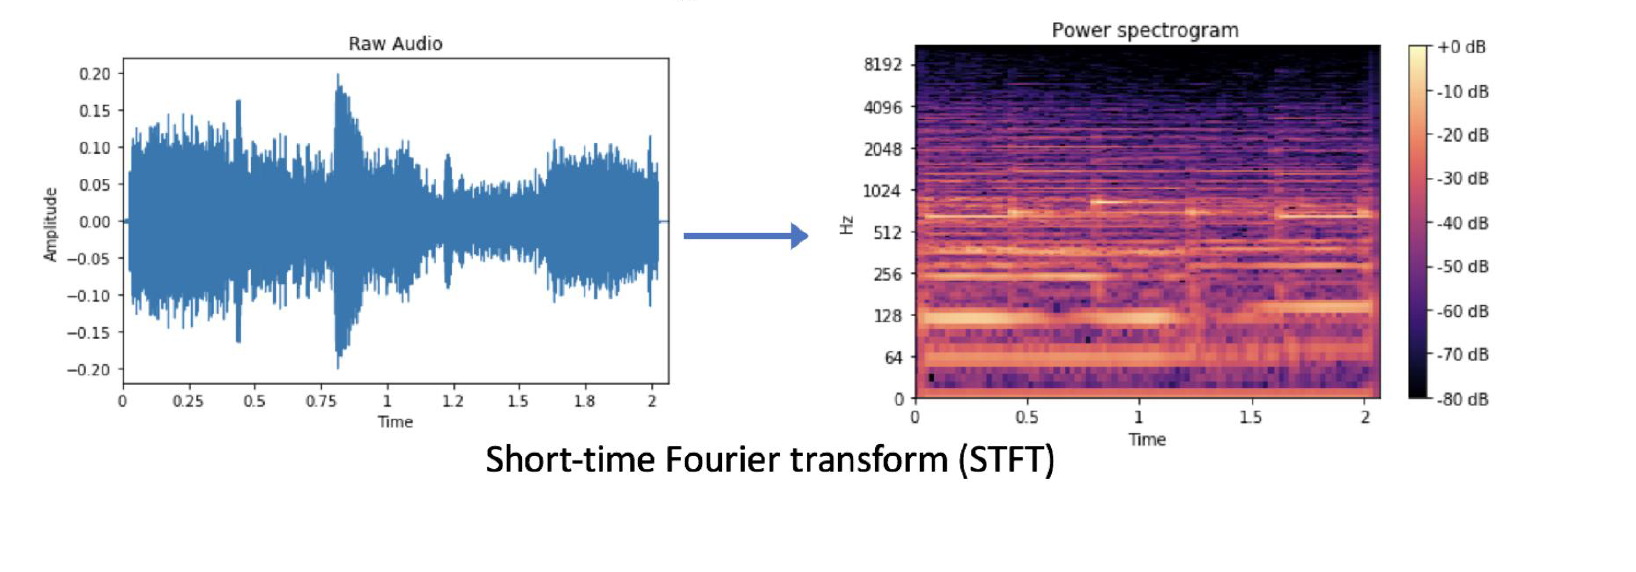
\includegraphics[scale=0.5]{stft.png}
}
\end{center}
   \caption{Raw Audio to 2-D Spectrograms}
\label{fig:short}
\end{figure*}

\subsubsection{Using a pretrained network}
Initially we built a shallow CNN which would accept content audio and style audio both converted to their respective audio spectrograms by STFT. We kept the weights of this network as constant and only updated the target audio iteratively. However the target output was not up to the mark and we could hear just the content audio with background noise in the target audio. Conventional neural transfer on images works by taking a pretrained network and then try to match the corresponding style and content target representations at these intermediate layers. Similarly we tried to use a pretrained network on audio samples. Here we observed that a pretrained network which is trained on images won't work on audio samples. Since images and audio are in a complete different domain, the initial layers of the network are unable to capture the low level features of audio spectrogram. Finally we created a deep neural network of 4 layers and trained on audio samples which are initially converted to audio spectrograms. We observed a significant improvement on the target audio generated by the network.



%------------------------------------------------------------------------
\section{Method and Proposed Architecture}
\subsection{Method}
In the first half of the project we implemented a base model as proposed by Leon Gatys and Matthias Bethge \cite{Authors00001}. We observed that the target audio generated was unable to capture the low level features of audio spectrograms. Hence the audio generated was unable match the features of the style audio. 
Later we used a shallow CNN to extract features of content and style audio. After training it up to 20000 iterations, we observed the total loss which is style loss plus content loss to be as shown in the Table 1. However the target audio generated was not up to the mark meaning the target audio has content audio mixed with background noise with very little features from the style audio. Meanwhile we also tried to use a pretrained model such as SoundNet which we found gave better results and inspired us to use a pretrained model. Our model was a 4 layer CNN model which we trained on audio spectrograms which was used to classify audio samples. We then used these weights to update our target audio while doing the optimization of target audio with respect to style and content audio.





\subsubsection{Style Transfer Algorithm}

\begin{figure*}
\begin{center}
\fbox{
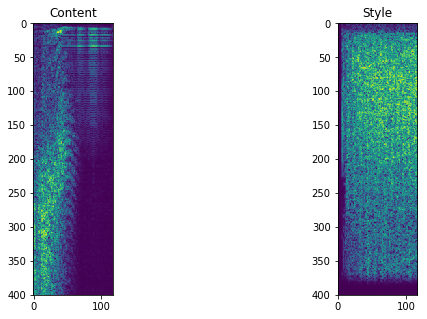
\includegraphics[scale=0.7]{inputs.png}
}
\end{center}
   \caption{Content and Style Spectrograms}
\label{fig:short}
\end{figure*}

The algorithm for neural style transfer used in this project is based on the Gatys et al\cite{Authors00001} approach, which involves taking one input as the content input and another as the style input, and generating a synthesized output containing content features from the content input and style features from the style input. See figure 2 for a diagram of the audio style transfer pipeline

To generate the synthesized output, we first obtain spectrograms from the content and style inputs via short-time fourier transform. Then we apply a shallow neural network to extract content features from the content spectrogram and style features from the style spectrogram. Content features are the activation's of first layer of the neural network. Style features for a given layer are the Gram Matrix of each filter’s activation, meaning that each filter’s activation is unrolled into a vector and then we compute the Gram Matrix of a matrix where each row is an unrolled filter activation. This results in a matrix of filter correlations. If there are multiple layers in the network then this Gram matrix is 
computed for each layer.

The next step is the optimization loop, which begins with initializing the output spectrogram randomly or as the content spectrogram, and then extracting content and style features from the output spectrogram to compare to the desired content and style features and compute loss. To calculate loss, we define the content features of the content input as Ccontent, the style features of the style input as S'style, and the content and style features of the generated output as Gcontent and G'style respectively. We define the content loss  and style loss as

Loss_Content = (C_content - G_Content)

Loss_Style = (S_Style - C_Style)
 
If there are multiple layers in the network then this style loss is averaged over the multiple layers to be consistent with Gatys et al. The total loss is computed as a weighted average of style loss and content loss.

With the loss calculation above, we update the generated output spectrogram using the Adam optimizer \cite{Authors00008}and repeat the extraction of content and style features, compute loss, and update again. This loop continues until the output converges to a spectrogram which contains the content features of the content input and the style features of the style input. The final step is to use the Griffin-Lim algorithm\cite{Authors00004} to convert the output spectrogram into raw audio.

\subsection{Architecture}
Our proposed architecture will have two steps. Step 1 will involve preprocessing of raw audio files. Content and style audio files will be converted to 2-D spectrogram by short time fourier transformation. We have used the librosa library to sample audio files in 2048 FFT window size.
We will then pass the content and style spectrogram into our model to extract style and content features. Step 2 will involve initializing the target audio with content audio (we also tried initializing it with random noise but the latter performed better) and then minimizing the overall cost which is a summation of L2 loss between content audio and L2 loss between gram matrix of style audio. For now we have used a shallow CNN model to test on instrumental music files. Later on we will implement a deeper layer CNN model to test its performance over larger music files.

\subsection{Innovation}


\begin{figure*}
\begin{center}
\fbox{
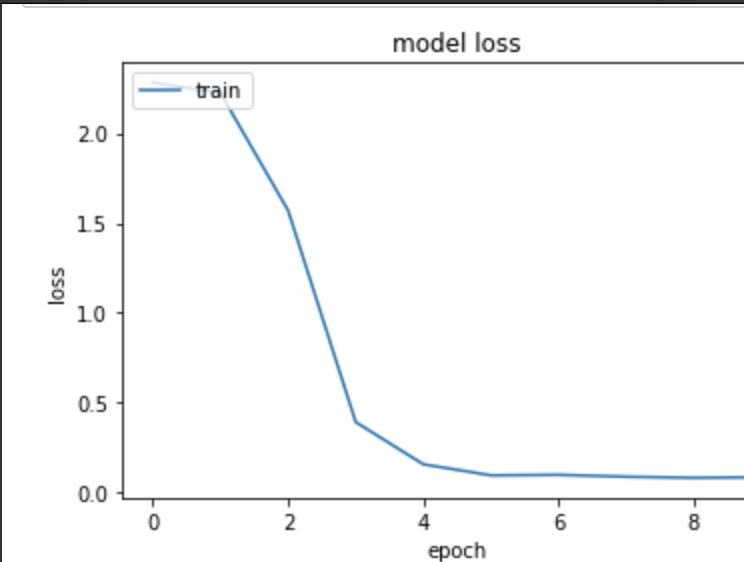
\includegraphics[scale=0.7]{train_loss.png}
}
\end{center}
   \caption{Training Loss}
\label{fig:short}
\end{figure*}

Since the above method of extracting features from style and content audio didn't give good results, we trained a CNN network having a deep layered architecture. This network was trained on audio spectrograms which is used for classification of audio signals. Similar to neural style transfer which uses activations from a pretrained network , we trained a network on audio spectrograms and then used these activations to make the content audio match with that of style audio. This allowed us to capture some of the low level features of audio signals and we observed some noticeable improvements to the target audio which was generated earlier without using a pretrained network.




\section{Results}

\begin{figure*}
\begin{center}
\fbox{
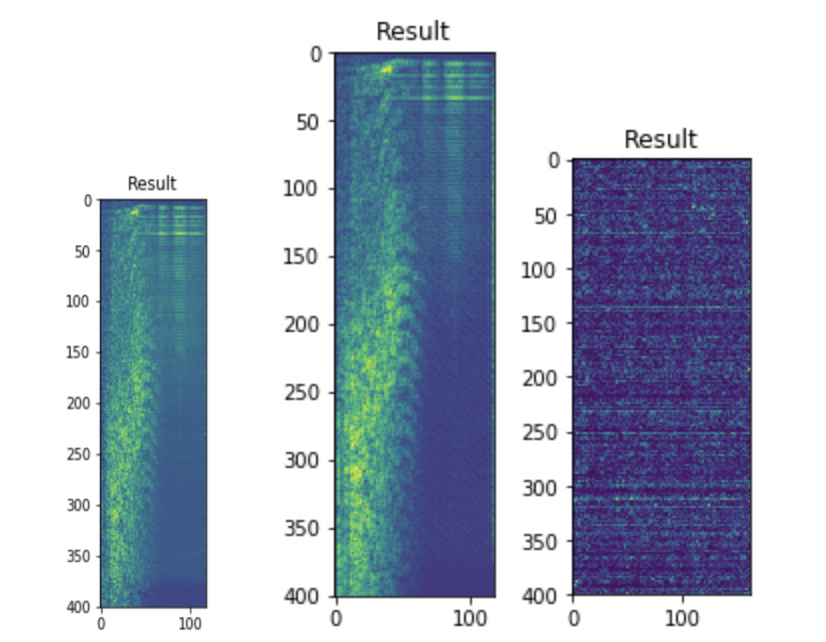
\includegraphics[scale=1.0]{all_results.png}
}
\end{center}
   \caption{Trained Model Results of trained, shallow and base models respectively}
\label{fig:short}
\end{figure*}

\subsection{Base Model}
We implemented the base model following the archtiecure proposed by Leon Gatys and Matthias Bethgev \cite{Authors00001}. The results are as shown in the Figure 5.
As seen from the audio spectrogram of the target audio, the resultant target audio shows little resemblance of content and style audio and is filled with noise. The model fails to learn features os content and style hence unable to produce a good representation of style and content audio.


\subsection{Shallow Model}
The results of the base model were not satisfactory. We tried a shallow CNN to extract style and content features and then used the style transfer algorithm to iteratively update the target audio. The target audio spectrogram is as shown in the Figure 5 which has some improvement over the base model.


\subsection{Deep Model with pretrained network}
Finally we trained a deep 4 layered CNN model on audio spectrograms giving it the task of audio classification. We then used these trained weights to further update the target audio using the style transfer algorithm. The training loss while training and the generated target audio is as shown in the Figure 5.

\section{GitHub Repository}
The github repository can be found at https://github.com/durvesh123/AudioStyleTransfer







%-------------------------------------------------------------------------

\begin{table}
\begin{center}
\begin{tabular}{|1|c|}
\hline
Iterations & Total Loss (Content loss + Style Loss) \\
\hline\hline
10000 & 130.50 \\
12000 & 113.23 \\
15000 & 100.89\\
20000 & 80.91\\
\hline
\end{tabular}
\end{center}
\caption{Preliminary Results}
\end{table}

%-------------------------------------------------------------------------



%-------------------------------------------------------------------------



%-------------------------------------------------------------------------


%-------------------------------------------------------------------------



%-------------------------------------------------------------------------


%------------------------------------------------------------------------


{\small
\bibliographystyle{ieee}
\bibliography{egbib}
}

\end{document}
